\documentclass{article}
\usepackage[T1]{fontenc}
\usepackage{lmodern}
\usepackage{graphicx}
\usepackage{amsmath,amssymb}
\usepackage[a4paper,margin=2cm]{geometry}
\usepackage[absolute,overlay]{textpos}
\setlength{\TPHorizModule}{1mm}
\setlength{\TPVertModule}{1mm}
\usepackage[indonesian]{babel}
\usepackage{hyperref}
\setlength{\emergencystretch}{2em}
% unit: Halaman 12

\begin{document}

% === Halaman 12 (llm) ===

\begin{center}
\textbf{Mode ECB}
\end{center}

\vspace{139.59mm}

E: Encryption \hfill D: Decryption \\
P$_i$: Plaintext block $i$ \hfill C$_i$: Ciphertext block $i$ \\
K: Secret key

\vspace{10mm}

% deskripsi: Diagram proses enkripsi dan dekripsi menggunakan mode Electronic Codebook (ECB), yang menunjukkan pengolahan blok plaintext menjadi ciphertext dan sebaliknya menggunakan kunci rahasia K.
% bbox normalisasi: [0.0000, 0.3800, 0.9600, 0.8500]
\begin{textblock*}{201.60mm}(0.00mm,112.86mm)
\noindent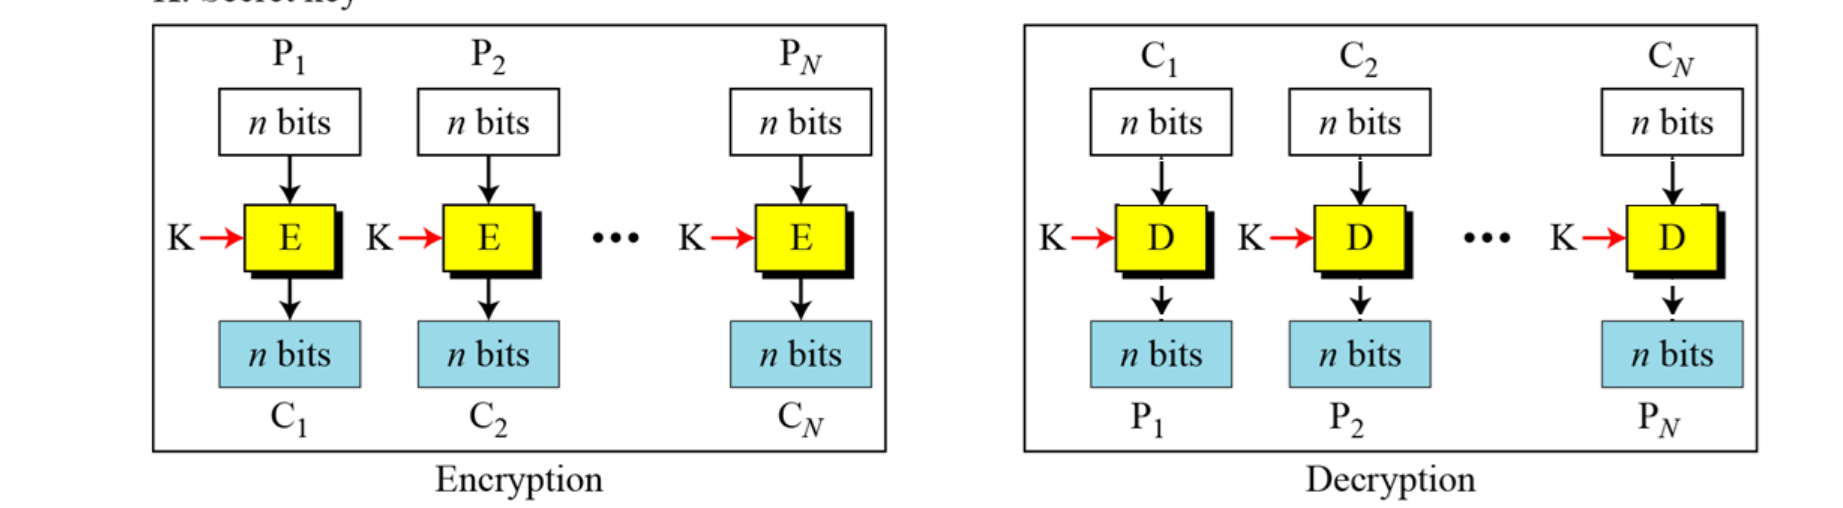
\includegraphics[width=201.60mm,height=139.59mm]{../../images/llm/page_012_img_01.png}%
\end{textblock*}

\end{document}
